\section{Results: Systematic Literature Review}
\label{section:Results_SLR}

Using a systematic literature review (SLR), following the method described, to answer the question, ``What is the current state of Projectional Editing'', leads us to the conclusion of - undetermined.

We make this statement because the review design was not appropriate for the problem domain.
The SLR was abandoned after the quality assessment stage.
We were unable to find a quality assessment checklist that adequately accounted for action design research, which most of the primary studies were.
There were some self-identified case studies which in fact were only descriptions of usage of implementations, rather than case studies in a scientific sense.

Therefore what follows should be considered as the results of a Quasi-SLR.

\subsection{Papers Selected}
The details of what is described in this section are logged in appendix \ref{Appendix:SLRLog}

Figure \ref{fig:search_results} shows the results of the 5 iterations that the search went through.
From our initial search using the scholarly search tools out of 173 results we had 50 papers that initially seemed to pass our inclusion and exclusion criteria.
From the initial 50, we added 18 papers from a possible 109 in our first iteration of forward and backward snowballing.
The next snowballing iteration returned three papers that matched our criteria.
The third round of snowballing had no matching papers and thus terminated this stage of selection.

\begin{figure}[htbp]
    \centering
    \fbox{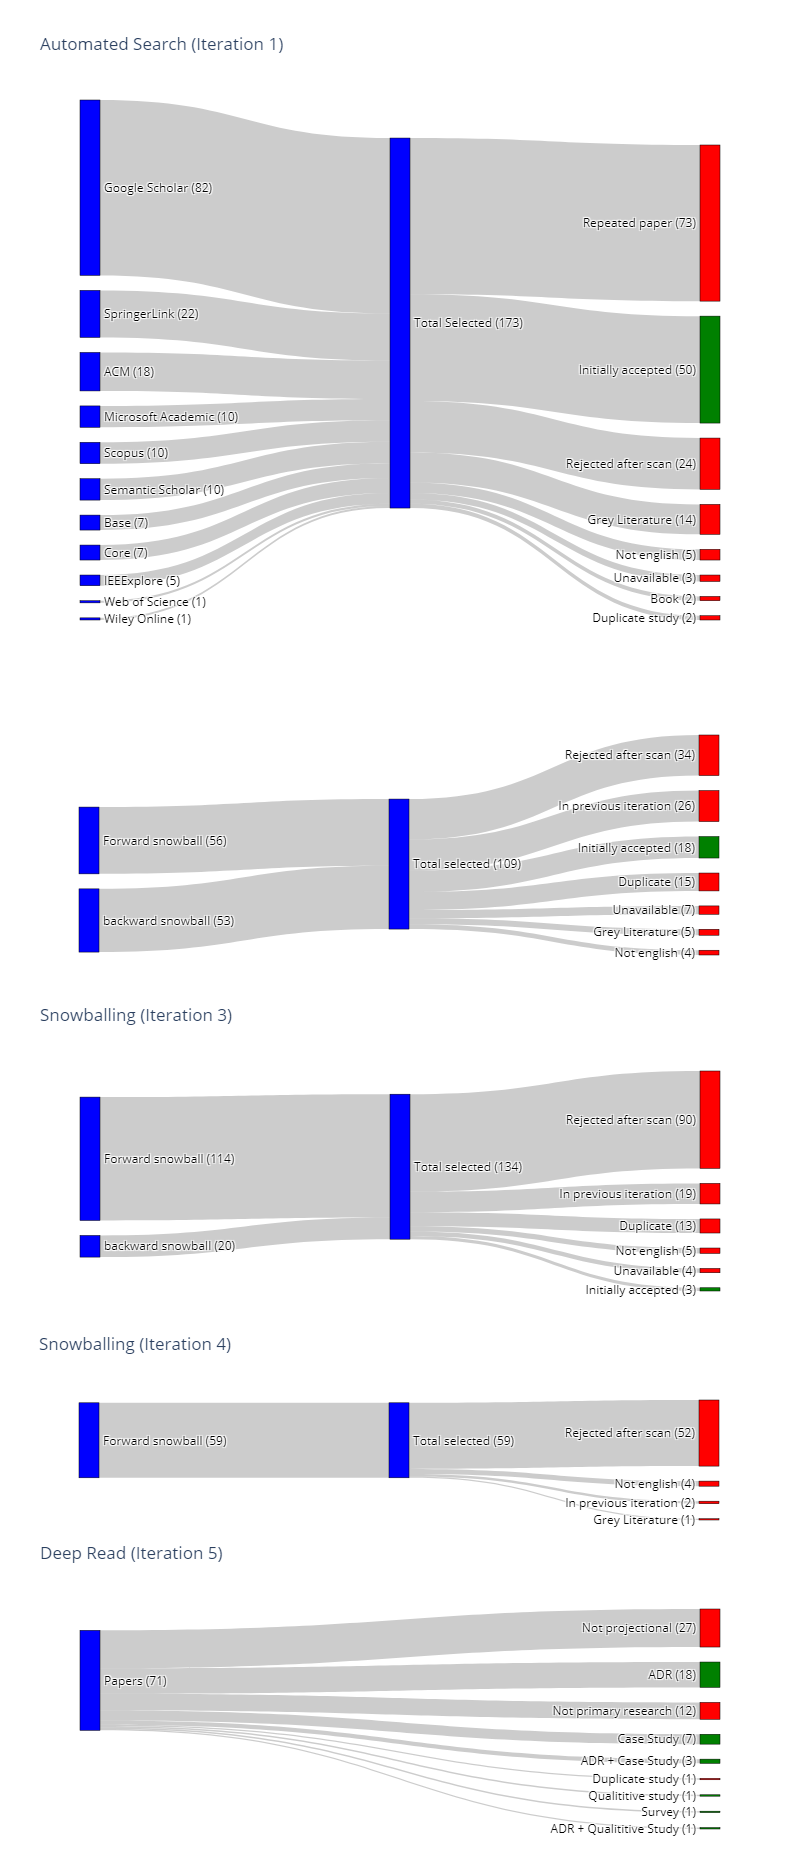
\includegraphics[width=0.75\textwidth]{/Sections/images/search_sankey.png}}
    \caption{Search results}
    \label{fig:search_results}
\end{figure}


Our final selection iteration involved a deeper scan of to determine of the remaining 71 papers.
With this we could reject 12 papers which were not primary research, one paper that reported a study already represented.
There were also 27 papers that were, on closer reading, not about projectional editing.

This left us with 31 papers before the quality assessment filter.

\subsubsection{Sensitivity and Precision}
As a curio, we reapproriated Zhang's\cite{Zhang_2011} ideas of sensitivity and precision and applied them to the search engines rather than search strings.
The values for sensitivity and precision of the search engines are calculated as follows:
\[
        sensitivity = \frac{\#\;retrieved\;relevant\;studies}{all\;relevant\;studies} \;100\%
\]

\[
        precision = \frac{\#\;retrieved\;relevant\;studies}{\#\;studies\;retrieved} \;100\%
\]

Table \ref{table:sensitivity_precision} show that Google Scholar had the highest sensitivity, returning 22 of the 31 chosen studies.
This came at the cost of a very large proportion of false positives.
Microsoft Academic and SpringerLink were joint most precise with half of their search results ending up in the final roster.
SpringerLink, with the second highest count of documents, second highest sensitivity, and joint highest precision would appear to be the best all around search engine for this field.
However, these figures are skewed by several of their articles coming from a single collection specifically about projectional editing.

\begin{table}[h]
    \begin{center}
        \begin{tabular}{ | l | c | c | c | c |} 
            \hline
            Search engine/library     & original \# & selected \# & sensitivity & precision\\
            \hline
            \hline
            ACM                        & 18          & 3           & 10\%        &  16\%    \\
            BASE                       & 7           & 3           & 10\%        &  43\%    \\
            CORE                       & 7           & 1           &  3\%        &  14\%    \\
            Google Scholar             & 82          & 22          & 71\%        &  27\%    \\
            IEEExplores                & 5           & 2           &  6\%        &  40\%    \\
            Microsoft Academic         & 10          & 5           & 16\%        &  50\%    \\
            Science.gov                & 0           & 0           &  0\%        &   0\%    \\
            SCOPUS                     & 10          & 3           & 10\%        &  30\%    \\
            Semantic Scholar           & 10          & 4           & 13\%        &  40\%    \\
            SpringerLink               & 22          & 11          & 35\%        &  50\%    \\
            Wiley Online               & 1           & 0           &  0\%        &   0\%    \\
            Web of Science             & 1           & 0           &  0\%        &   0\%    \\
            \hline
        \end{tabular}
    \end{center}
    \caption{Search engine sensitivity and precision}
    \label{table:sensitivity_precision}
\end{table}


\subsection{Quality Assessment}
Using the quality assessment checklists, developed by Crombie et al.\cite{crombie1997pocket}, shown in appendix \ref{appendix:QualityAssesmentChecklist} we examined the remaining 31 papers which on the surface represented 37 primary studies.
As action design research was not represented amongst these checklists we searched for an appropriate quality assessment checklist for these type of primary study.
We did not find a suitable checklist, and did not consider ourselves suitably qualified to make one.
Thus we used the case study quality assessment checklist to assess the ADR studies.

We used a rudimentary scoring system of +1 value for positive answers, 0 for ``don't knows'', and -1 for negative answers.
We arbitrarily chose that any study with an overall score greater than 0 would be considered high enough quality to be part of our final analysis.

With this scoring and goal we only found 6 out of 37 studies of high enough quality.

We therefore had to decide to change our scoring, go ahead with 6 studies, stop here or ignore the QA findings.
Changing the scoring until you get the ``right'' result felt wrong.
6 studies seems too few to give an overview of a field.
Stopping seems to be the correct course for an SLA.
However, we decided to create a new Quasi-SLA, that ignores the results of a Quality assessment.

Our reason to continue was that we could not reconcile that 84\% of studies that had made it to the recognized scientific journals were not of high enough quality to pass our SLR QA stage.
We believe there were two large threats to the validity of the Quality Assessment stage that were too great to ignore.
The first being that it was carried out by a single researcher with no previous experience.
The other being either that the use of case study checklists is inappropriate for ADR studies or that ADR studies are inappropriate for SLRs.


\subsection{Analysis}
After Identifying the primary studies we extracted data, the details of which are shown in appendix \ref{appendix:DataExtraction}.
Figure \ref{fig:study_types} shows that most of the primary studies in our review were ADR studies.

\begin{figure}[h]
    \centering
    \fbox{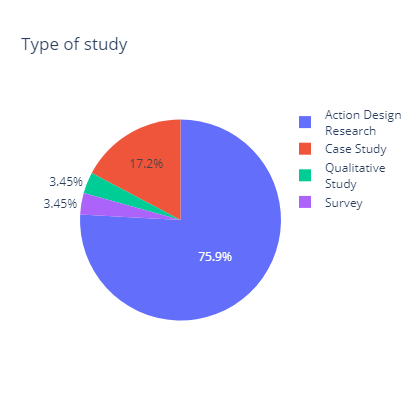
\includegraphics[width=0.35\textwidth]{/Sections/images/pie_study_type.png}}
    \caption{Study types}
    \label{fig:study_types}
\end{figure}

\subsubsection{Tools used}
We split the studies to see which were to do with purely research projects and which were researching using already publicly available commercial or opensource products.
To calculate this we removed the one Primary study that was a survey, as it covered a multitude of tools and options, none of which in depth.\
The chart in figure \ref{fig:public_vs_research} shows that over 80\% of the projects were studying already existing publicly available options.

Of the studies that using on publicly available software, we wanted to know what software was attracting most academic interest.
Figure \ref{fig:public_programs} shows that 74\% of the studies into projectional editing that were using a publicly available product were conducted using Jetbrains.

\begin{figure}
    \centering
    \fbox{\begin{minipage}{0.47\textwidth}
            \centering
            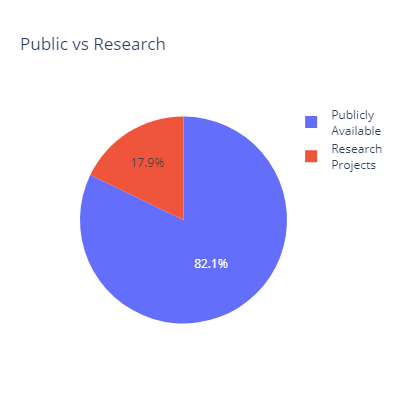
\includegraphics[width=0.85\textwidth]{Sections/images/pie_projectional_publicvsresearch.png}
            \caption{Public vs research}
            \label{fig:public_vs_research}
        \end{minipage}\hfill
        \begin{minipage}{0.53\textwidth}
            \centering
            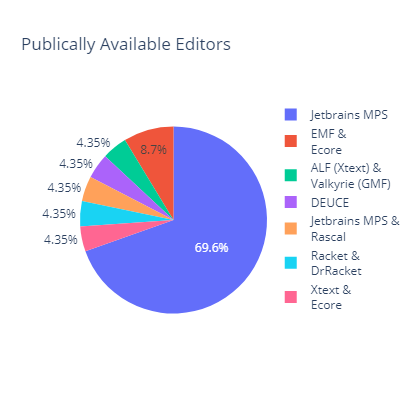
\includegraphics[width=0.85\textwidth]{Sections/images/pie_projectional_publicprograms.png} 
            \caption{Publicly available programs}
            \label{fig:public_programs}
        \end{minipage}
    }
\end{figure}

\subsubsection{Sentiment}

In this study we included all 29 papers.
We tagged each section from those papers that talked about projectional editing.
We then broke each of these sections into sentences and ran those sentences through a sentiment analyser as described in section \ref{section:dataExtraction}.
The outcome of these are shown in figure \ref{fig:sentiment_analysis}.

The charts show the relationship between the positive, neutral and negative sentiment outcomes.
On the y-axis, we have an Id for the papers being examined. 
A key linking the Id to the paper name is seen in table \ref{table:paper_key};

The first chart shows the absolute number of sentences that were analysed per paper partitioned by whether they returned negative, neutral and positive.
The second chart shows these as percentages, so that the papers are more comparable.
In the third chart we removed the neutral scores and calculated the percentage positive to negative.
The final chart is an aid to make it easier to scan whether papers were more positive, more negative.
If we found the papers to be equally positive and negative, we classified them as neutral.

Over the 29 papers we scanned a total of 3003 sentences.
435 were analysed as being positive, 1953 neutral and 615 negative.
Thus 14\% were positive and 16\% negative.

10 of the 29 papers were more positive than negative when talking about projectional editing, 16 more negative and 3 equally negative and positive.

In figure \ref{fig:sentiment_analysis2} we attempt to separate out sentiment by product category.  
These categories being Research projects, MPS and all the other used products.
We ignored the survey paper in this one as it covered all of these types.

As MPS dominates the sentences accounting for 17 (61\%) of the 28 papers and 2051 (73\%) of the 2791 sentences analysed, the comparison does not give much value.

\begin{figure}[h]
    \centering
    \fbox{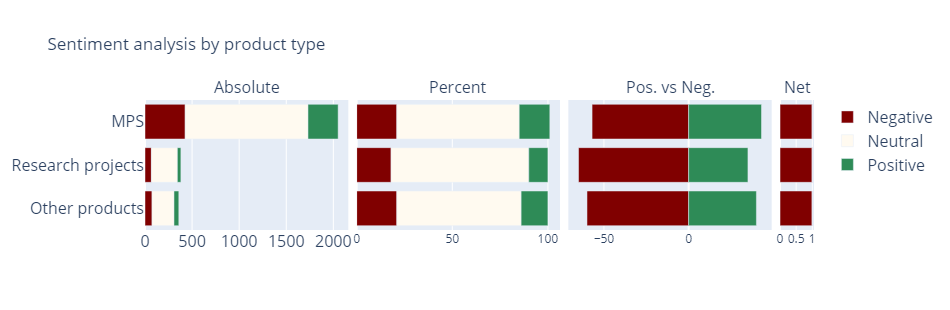
\includegraphics[width=0.95\textwidth]{/Sections/images/sentiment_analysis2.png}}
    \caption{Sentiment analysis by product}
    \label{fig:sentiment_analysis2}
\end{figure}

\begin{figure}[htbp]
    \centering
    \fbox{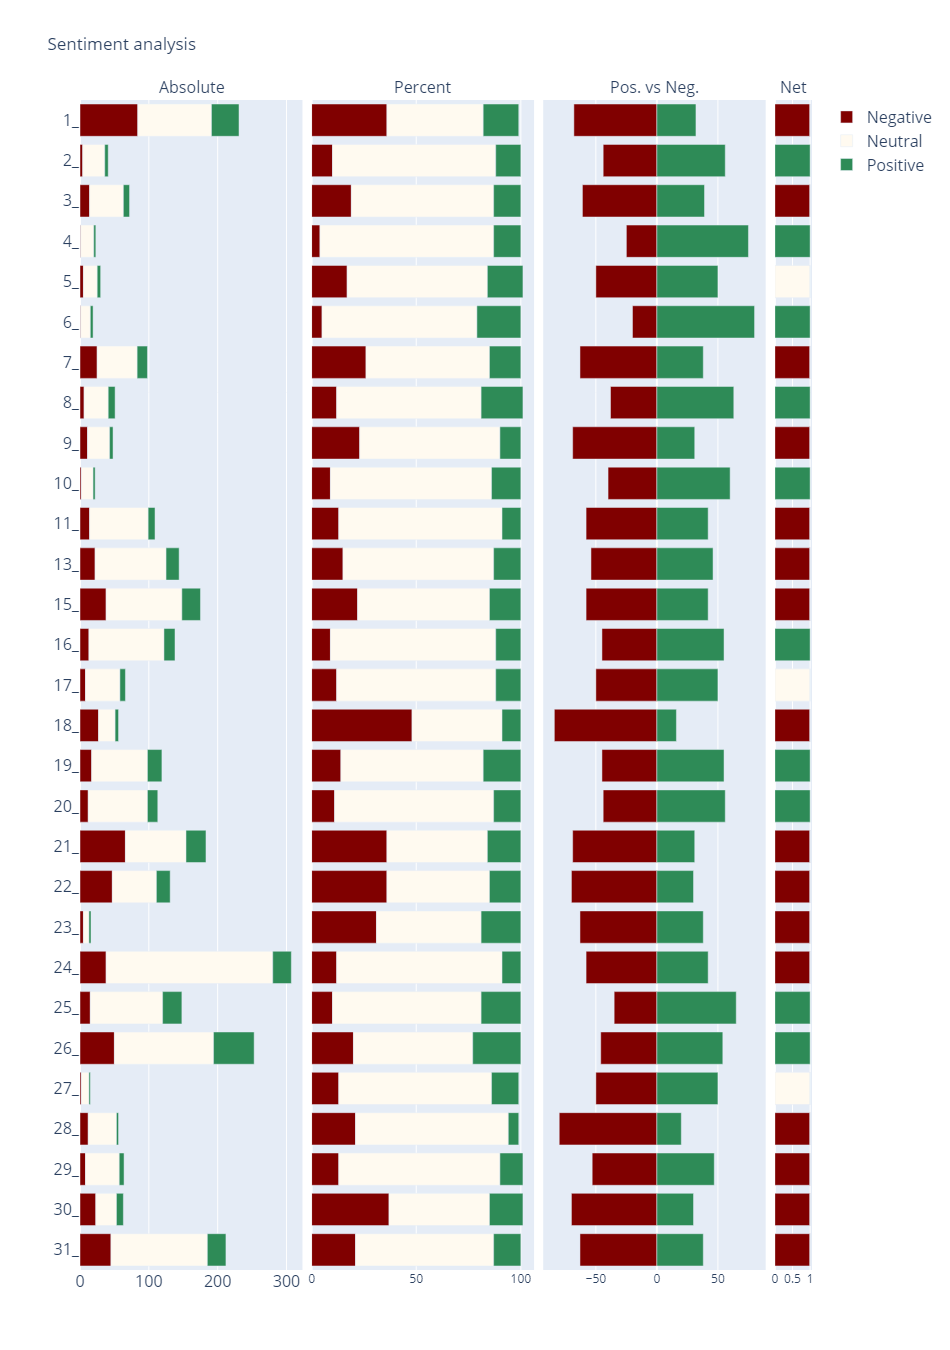
\includegraphics[width=0.95\textwidth]{/Sections/images/sentiment_analysis.png}}
    \caption{Sentiment analysis}
    \label{fig:sentiment_analysis}
\end{figure}


\begin{table}[htbp]
    \begin{center}
        \begin{tabular}{ |c  c|l | } 
            \hline
            Id  &                                        & Paper name                                                                  \\
            \hline
            1   &  \cite{voelterdomain_SLR}              & A domain-specific language for payroll calculations: A case study at DATEV  \\ \hline
            2   &  \cite{schropfer2021framework_SLR}     & A framework for projectional multi-variant model editors                    \\ \hline
            3   &  \cite{schropfer2020generic_SLR}       & A generic projectional editor for EMF models                                \\ \hline
            4   &  \cite{bucchiarone2019model_SLR}       & A model-driven approach towards automatic migration to microservices        \\ \hline
            5   &  \cite{meacham2020adaptivevle_SLR}     & AdaptiveVLE: An integrated framework for personalized online education      \\
                &                                        & using MPS JetBrains domain-specific modeling environment                    \\ \hline
            6   &  \cite{andersen2020adding_SLR}         & Adding interactive visual syntax to textual code                            \\ \hline
            7   &  \cite{addazi2021blended_SLR}          & Blended graphical and textual modelling for UML profiles: A                 \\
                &                                        & proof-of-concept implementation and experiment                              \\ \hline
            8   & \cite{meacham2020classification_SLR}   & Classification algorithms framework (CAF) to enable intelligent systems     \\
                &                                        & using JetBrains MPS domain-specific languages environment                   \\ \hline
            9   & \cite{furtado2021dsl_SLR}              & DSL based approach for building model-driven questionnaires                 \\ \hline
            10  & \cite{beckmann2020efficient_SLR}       & Efficient editing in a tree-oriented projectional editor                    \\ \hline
            11  & \cite{kolovos2020efficient_SLR}        & Efficient generation of graphical modelviews via lazy model-to-text         \\
                &                                        & transformation                                                              \\ \hline
            13  & \cite{bucchiarone2021engineering_SLR}  & Engineering gameful applications with MPS                                   \\ \hline
            15  & \cite{ratiu2021fasten_SLR}             & Fasten: An extensible platform to experiment with rigorous modeling of      \\
                &                                        & safety-critical systems                                                     \\ \hline
            16  & \cite{lafontant2020gentleman_SLR}      & Gentleman: A light-weight web-based projectional editor generator           \\ \hline
            17  & \cite{schropfer2019integrating_SLR}    & Integrating UML and ALF: An approach to overcome the code generation        \\
                &                                        & dilemma in model-driven software engineering                                \\ \hline
            18  & \cite{santos2020javardise_SLR}         & Javardise: A structured code editor for programming pedagogy in Java        \\ \hline
            19  & \cite{schindler2021jetbrains_SLR}      & Jetbrains MPS as core DSL technology for developing professional digital    \\
                &                                        & printers                                                                    \\ \hline
            20  & \cite{simi2021learning_SLR}            & Learning data analysis with metaR                                           \\ \hline
            21  & \cite{stotz2021migrating_SLR}          & Migrating insurance calculation rule descriptions from Word to MPS          \\ \hline
            22  & \cite{munk2020model_SLR}               & Model-based safety assessment with sysml and component fault trees:         \\
                &                                        & Application and lessons learned                                             \\ \hline
            23  & \cite{bucchiarone2020papyrus_SLR}      & Papyrus for gamers, let’s play modeling                                     \\ \hline
            24  & \cite{merino2021projecting_SLR}        & Projecting textual languages                                                \\ \hline
            25  & \cite{cuinat2020specedit_SLR}          & SpecEdit: Projectional editing for TLA+ specifications                      \\ \hline
            26  & \cite{prinz2021teaching_SLR}           & Teaching language engineering using MPS                                     \\ \hline
            27  & \cite{barash2021teaching_SLR}          & Teaching MPS: Experiences from industry and academia                        \\ \hline
            28  & \cite{hempel2020tiny_SLR}              & Tiny structure editors for low, low prices! (generating guis from           \\
                &                                        & toString functions)                                                         \\ \hline
            29  & \cite{negm2020towards_SLR}             & Towards ontology-based domain specific language for internet of things      \\ \hline
            30  & \cite{lubin2020type_SLR}               & Type-directed program transformations for the working functional            \\
                &                                        & programmer                                                                  \\ \hline
            31  & \cite{ozkaya2021practitioners_SLR}     & What do practitioners expect from the meta-modeling tools? a survey         \\ \hline
        \end{tabular}
    \end{center}
    \caption{paper key}
    \label{table:paper_key}
\end{table}

\subsubsection{A Narrative Synthesis}
Our synthesis of the papers that appear in table \ref{table:paper_key} will be short.
We will avoid rehashing the advantages and disadvantages of projectional editing, as discussed in sections \ref{section:projectional_advantages} and \ref{section:projectional_disadvantages}.

There is much focus in these papers on models, and model driven development.
Some mention is made of a shift towards textual modelling languages.
However, others point out that the suitable level of abstraction is not always found in text.

When authors have used solutions other than MPS, they complain about issues such as MPS being heavy-weight, with a lot of overhead.
However, these authors then spend a great deal of time theorising about how to fix issues that are fixed by default in the implementation of MPS.
The projects they describe are not in industrial use.
These authors think that projectional editing is probably best suited to helping novices learn a language. 

There is a fair bit of mention of ``semi-projectional'' approach, where there is parsing at the leaf level.
This is mainly from those who don't use MPS, but also some who do.
This, it seems, is a reaction to the difficulty in simulating the text language experience in a projectional editor.

Those authors who use MPS are mostly either discussing products developed for use in an industrial setting or discussing how best to teach projectional editing.
When MPS is used it is often seen as a key enabler.

The
